\documentclass[Afour,sageh,times]{sagej}
% Shared mathematical and layout conventions; the SAGE class is unmodified.
\usepackage{fontspec}
\setmainfont{NimbusRoman-Regular.otf}[BoldFont=NimbusRoman-Bold.otf,ItalicFont=NimbusRoman-Italic.otf,BoldItalicFont=NimbusRoman-BoldItalic.otf]
\setsansfont{NimbusSans-Regular.otf}[BoldFont=NimbusSans-Bold.otf,ItalicFont=NimbusSans-Italic.otf,BoldItalicFont=NimbusSans-BoldItalic.otf]
\setmonofont{DejaVu Sans Mono}[Scale=0.78]
\usepackage{mathtools,tabularx,array,etoolbox}
\usepackage[unicode,colorlinks=true,linkcolor=blue,citecolor=blue,urlcolor=blue]{hyperref}
\urlstyle{same}
\setcounter{secnumdepth}{2}
\setcounter{tocdepth}{2}
\setlength{\emergencystretch}{1em}
\newtheorem{proposition}{Proposition}
\newtheorem{theorem}{Theorem}
\newtheorem{lemma}{Lemma}
\newtheorem{remark}{Remark}
\newcommand{\R}{\mathbb R}
\newcommand{\StageBase}{1c73a580441200d6594e2a2a96374edc1c0e98e6}
\def\journalname{IJRR research manuscript}
\def\volumenumber{Draft}
\def\issuenumber{2026}
\def\volumeyear{2026}
% Remove publication metadata placeholders in the document, not in sagej.cls.
\makeatletter
\patchcmd{\@maketitle}{\hbox{}\volumenumber(\issuenumber):\startpage--\endpage\\}{\hbox{}Unsubmitted manuscript\\}{}{\PackageError{paper}{Title metadata patch failed}{}}
\patchcmd{\@maketitle}{\hbox{}\copyright The Author(s) \volumeyear\\}{\hbox{}Authors to be confirmed\\}{}{\PackageError{paper}{Author metadata patch failed}{}}
\patchcmd{\@maketitle}{\hbox{}Reprints and permission:\\}{\hbox{}Prepared for IJRR\\}{}{\PackageError{paper}{Submission metadata patch failed}{}}
\patchcmd{\@maketitle}{\hbox{}sagepub.co.uk/journalsPermissions.nav\\}{}{}{\PackageError{paper}{Permissions metadata patch failed}{}}
\patchcmd{\@maketitle}{\hbox{}DOI: 10.1177/ToBeAssigned\\}{\hbox{}No DOI assigned\\}{}{\PackageError{paper}{DOI metadata patch failed}{}}
\makeatother

\runninghead{Local structure and full-coil control of a magnetic rod}
\hypersetup{pdftitle={Local Birkhoff structure and full-coil control of a three-dimensional magnetic rod},pdfauthor={Authors to be confirmed}}
\title{Local Birkhoff structure and full-coil control of a three-dimensional magnetic rod}
\author{[Author names, affiliations and corresponding author to be supplied]}
\begin{document}
\begin{abstract}
Geometric integration and learned Hamiltonians can support magnetic soft-robot simulation only when they represent the same mechanical dynamics and realizable inputs. We study this interface on a three-dimensional Kirchhoff reduction with 12 configuration coordinates, configuration-dependent inertia, and full Biot--Savart coil forces. A transported one-form, a computable local Moser chart, and compatible endpoint generators separate structural matching from approximation of the original field. Higher transport order reduces the continuous representation gap, but does not consistently improve total integration error. On a fixed-current conservative branch, a nonseparable central generating method exhibits fourth-order convergence; smooth feedback and sampled constrained control require different structural claims. Energy differentiation and virtual work agree for the full-coil port, whereas a local affine field gives approximately 98.6\% force discrepancy in the tested configuration. Frozen complex-network comparisons expose a trade-off between field accuracy and positive momentum curvature. Three-dimensional resonance calculations retain non-action quartics and do not establish a KAM certificate. Transfer to a spatial Cosserat rod demonstrates constrained execution with prescribed flow and contact, but no tracking improvement. The results provide a reproducible, explicitly local connection between mechanics, structure and actuation, together with the limits of its present validation.
\end{abstract}
\keywords{magnetic soft robotics; Cosserat rods; Birkhoff systems; geometric integration; Hamiltonian learning; constrained magnetic control}
\maketitle
\section{Introduction}
Magnetic actuation can apply forces and torques to a slender robot without a distal motor. Its attraction for vascular intervention is accompanied by a difficult modeling requirement: the shape, material orientation, surrounding fluid and actuator geometry jointly determine the motion. A long-term application considered here is a three-dimensional flexible intravascular robot under space-station microgravity. Removing a dominant gravitational load does not remove blood-flow forcing, wall interaction, magnetic workspace limits or rotational inertia. The present study addresses the mathematical and computational interfaces needed for this application; its evidence consists of simulations and local analysis, rather than physiological or clinical validation.

A structure-preserving update is useful only after specifying the dynamics whose structure it preserves. A canonical Hamiltonian reduction supplies one such structure on a conservative branch. Nonconservative loads generally invalidate its preservation. A time-dependent Birkhoff form can represent a smooth loaded field locally, but an approximate transported form may represent a nearby field instead. Likewise, a learned scalar energy defines a conservative predictor, while a magnetic actuator can apply only a restricted momentum force. Confusing these objects can produce a small structural defect alongside an inaccurate physical trajectory. The distinction is particularly consequential for a three-dimensional rod with configuration-dependent mass and spatially varying coil fields.

We study these interfaces on a geometric Kirchhoff reduction, with two bending directions and twist, and use a spatial Cosserat model to examine environmental transfer. The reduction retains 12 configuration variables and all derivatives of its mass matrix. A full Biot--Savart energy provides the current-to-generalized-force map. Local one-form transport, Moser charts and endpoint generators are then evaluated on declared smooth branches. Hamiltonian learning and resonance diagnostics share the ideal-bias conservative reduction; the full-coil closed loop is identified separately. The paper consequently reports connected model interfaces with explicit scope, rather than a single experiment combining every method.

The contribution has three parts. First, we give a computable local connection from this variable-inertia rod field to a transported two-form and compatible generating update, retaining representation, chart, integration and solver errors as distinct quantities. The derivation specifies endpoint transversality, initial gauge and fixed-coordinate recursion, and recovers a nonseparable fourth-order central method on the autonomous conservative branch. These are applications and explicit compatibility statements within established geometric mechanics, not claims to originate Darboux or generating-function theory. Second, we connect magnetic potential, virtual work, feedback differentiation and constrained allocation to the same geometric reduction, and quantify the failure of a local affine field on the tested coil geometry. Third, we report the limits of learning, resonance and spatial-rod transfer: good sampled field prediction need not give positive momentum curvature; a nonzero formal resonant twist is not a KAM certificate; and feasible port execution need not improve tracking.

\section{Related work and relation to the research record}
Geometrically exact rod models distinguish centerline deformation from material-frame rotation. Their variational and computational foundations are described by \citet{Antman2005,Simo1985}; \citet{Gazzola2018} develop forward and inverse soft-filament mechanics. These models justify retaining shear/stretch in a full Cosserat calculation while imposing an explicit Kirchhoff restriction in a lower-dimensional analytical model. Magnetic methods and workspace-dependent actuation are reviewed by \citet{Abbott2020}. Ferromagnetic continuum robots illustrate the physical platform \citep{Kim2019}, while confined-lumen magnetic-robot simulation and navigation motivate the parameter and implementation lineage used here \citep{Tong2025}. Our coil array and residual-acceleration prescription remain benchmark choices rather than measured hardware or microgravity physiology.

Generating functions provide canonical difference schemes \citep{Feng1989}, and the broader theory of symplectic algorithms is developed by \citet{FengQin2010,Hairer2006}. Birkhoffian schemes extend the structural question to a noncanonical two-form \citep{Su2007}. For dissipative physical dynamics, the time compatibility of that form is essential: spatial closedness alone does not establish a representation of the supplied vector field. We use an auxiliary Moser flow to compute a local chart, retaining its time derivative. The original robot flow supplies a local existence argument but is not an available numerical input. The fourth-order formula in this paper is a central generating method for a nonseparable Hamiltonian, not a separable drift--kick composition.

Hamiltonian neural networks learn an energy whose derivatives define a field \citep{Greydanus2019}. Learning-to-KAM arguments require substantially stronger norm control and hypotheses than a finite test loss \citep{Chen2022}. Classical and finitely differentiable persistence results \citep{Poschel2001,Bounemoura2020}, and discrete results for symplectic algorithms \citep{Shang1999}, make those obligations explicit. In the present circular rod, four pairs of equal bending frequencies prevent direct reuse of a nonresonant two-mode certificate. We retain the existing finite-feature and statistical implications as conditional results and report the computed resonant terms without claiming a new invariant torus.

The evidence cutoff is the Stage~5 branch at repository commit \texttt{1c73a58}. The initial 1025 research manuscript supplies the physical and mathematical intent; the Stage~4 audit identifies corrections, and Stage~5 supplies their implementations and available validation. The present paper includes no Stage~6 or later bridge results and performs no new scientific simulation or training. Existing outputs are selected by their recorded validation status, with rejected derivative calculations and failed allocations retained as distinct evidence. The accompanying manifests map equations, numerical claims and figure series to exact source files and fields. This restriction matters: the same repository also contains historical two-mode and planar experiments whose existence does not establish a three-dimensional result.

\section{Three-dimensional mechanics and realizable magnetic control}
\label{sec:model-control}

\subsection{Two mechanical resolutions of the same robot}
The physical target is a flexible magnetic robot in a vessel under residual microgravity. Its centerline alone does not determine its state: material twist can change while the centerline remains straight. We therefore retain both the centerline $r(s,t)\in\mathbb R^3$ and material frame $R(s,t)\in SO(3)$, with reference arclength $s\in[0,L]$. The Cosserat strains and body angular velocity are
\begin{equation}
 \nu=R^Tr_s,\qquad \widehat\kappa=R^TR_s,\qquad
 \widehat\Omega=R^TR_t,
 \label{eq:rod-kinematics}
\end{equation}
where $\widehat a b=a\times b$. With internal force $n$, moment $m$, and external force and couple densities $f,\ell$, the balances read
\begin{equation}
\begin{aligned}
 \rho_s A r_{tt}&=n_s+f,\\
 R\bigl(J_b\dot\Omega+\Omega\times J_b\Omega\bigr)
 &=m_s+r_s\times n+\ell.
\end{aligned}
 \label{eq:rod-balance}
\end{equation}
Here $J_b$ is rotary inertia per reference length. The elastic laws use
$n=RK_s(\nu-e_3)$ and $m=RK_b\kappa$ for an initially straight rod, with
$K_b=\operatorname{diag}(EI_1,EI_2,GJ_p)$; $K_s$ denotes shear/stretch stiffness, and is unrelated to the Birkhoff two-form. These conventions keep both bending axes, torsion, and rotary inertia explicit \citep{Antman2005,Gazzola2018}.

We use two resolutions with different purposes. The spatial Cosserat model admits shear and extension and evaluates prescribed flow, wall contact, friction, magnetic loads, and residual acceleration. Its base node and first material frame are fixed and its distal end is free. The analytical model imposes the Kirchhoff constraint $\nu=e_3$ and expands each of the two bending strains and the twist strain in four normalized Legendre functions. It consequently has 12 configuration coordinates and 24 phase coordinates. Its 20, 40, or 80 spatial cells are quadrature cells, not additional configuration degrees of freedom. Exponential frame updates and midpoint centerline integration supply the actual three-dimensional embedding. The two models share material and magnetic parameters, but there is no established uniform error bound between them.

The benchmark has $L=100$\,mm, radius $0.6$\,mm, $E=3$\,MPa, $G=1$\,MPa, and density $1800$\,kg\,m$^{-3}$. The distal $5$\,mm carries body-aligned permanent magnetization with line dipole density $0.1448$\,A\,m, giving total moment $7.24\times10^{-4}$\,A\,m$^2$. The ideal axial bias is $0.5$\,mT. Material and magnet values are literature-informed benchmark inputs \citep{Tong2025}; assigning the same elastic constants along the complete shaft is a modeling assumption. Density, damping, coil ratings, wall parameters, and residual acceleration are engineering or synthetic choices, rather than measurements of an implanted device.

In the environmental model, the fluid density and viscosity are $1060$\,kg\,m$^{-3}$ and $3.5$\,mPa\,s. A prescribed curved-tube parabolic profile has centerline speed scale $0.04$\,m\,s$^{-1}$, pulsation fraction $0.45$, and frequency $1.2$\,Hz. Anisotropic linear relative drag, transverse quadratic drag including the rod diameter, and axial-spin drag are implemented. A dimensionally consistent Morison-type inertial extension would depend on fluid acceleration and relative acceleration; added mass is not implemented here. Prescribing fluid velocity can supply mechanical energy even when relative drag is dissipative. The lumen is rigid and stationary, with nominal radius $3$\,mm. Positive penetration $\delta_+$ generates contact potential density $k\delta_+^{5/2}/(5/2)$, supplemented by compressive normal damping and regularized tangential friction. Structural damping is $2$\,s$^{-1}$. Residual acceleration $(8,-5,2)\times10^{-5}$\,m\,s$^{-2}$ and $3\times10^{-5}$\,m\,s$^{-2}$ jitter with nominal frequency $3$\,Hz define a synthetic microgravity case. Neither this flow prescription nor the wall model constitutes two-way fluid--structure interaction.

\subsection{Canonical scaling without freezing inertia}
Let $q$ denote the physical Ritz coefficients. The embedding induces translational and body-angular velocity Jacobians $J_r(q,s)$ and $J_\Omega(q,s)$, hence
\begin{equation}
\begin{aligned}
 M(q)&=\int_0^L\left(\rho_s A J_r^TJ_r+
 J_\Omega^TJ_bJ_\Omega\right)\,ds,\\
 p&=M(q)\dot q.
\end{aligned}
 \label{eq:geometric-mass}
\end{equation}
All evaluations retain this configuration-dependent mass. In particular, the kinetic contribution to $\dot p_a$ is
$\tfrac12\dot q^T(\partial_{q_a}M)\dot q$; removing it changes the physical vector field.
The fixed scaling
\begin{equation}
\begin{gathered}
 q=S_qQ,\qquad p=S_pP,\\
 S_q^TS_p=\frac{E_0}{\omega_0}I,\\
 \tau=\omega_0t,\qquad h=H/E_0.
\end{gathered}
 \label{eq:canonical-scaling}
\end{equation}
gives $z=(Q,P)$, $z'=J\nabla h$, and
\begin{equation}
\begin{aligned}
 \overline M(Q)&=\frac{\omega_0^2}{E_0}S_q^TM(S_qQ)S_q,\\
 T/E_0&=\tfrac12P^T\overline M(Q)^{-1}P.
\end{aligned}
 \label{eq:scaled-mass}
\end{equation}
Primes denote differentiation with respect to $\tau$; $J=\left(\begin{smallmatrix}0&I\\-I&0\end{smallmatrix}\right)$.
For the default 20-cell geometry, $E_0=3.62\times10^{-7}$\,J and $\omega_0=4.4576294085$\,rad\,s$^{-1}$. The scaling is constructed from the ideal-bias linearization and then held fixed. It neither puts the full-coil system at equilibrium at $Q=0$ nor makes the ideal linear frequencies the frequencies of a new coil equilibrium. State norms below are dimensionless canonical norms; dimensional tip errors require geometric reconstruction.

The ideal-field branch uses $h_{\rm ideal}=(T+V_e+V_{\rm uniform})/E_0$, up to a constant. The full-coil branch instead uses
\begin{equation}
\begin{aligned}
 h_{\rm coil}(z,i)&=\tfrac12P^T\overline M^{-1}P\\
 &\quad+V_e(S_qQ)/E_0+\phi(Q)^Ti.
\end{aligned}
 \label{eq:coil-hamiltonian}
\end{equation}
The currents $i\in\mathbb R^{12}$ are total currents in amperes. Their pre-energized bias $i_b$ is fitted to the local axial target and has maximum magnitude $1.5124804$\,A. No additional ideal-bias potential is added to \eqref{eq:coil-hamiltonian}. Thus comparisons between ideal and coil branches change the physical potential, whereas comparisons of integrators within one branch keep that potential fixed.

\subsection{Full-coil energy, virtual work, and reachability}
The engineered air-core array contains twelve circular coils of radius $25$\,mm and 300 turns, centered $75$\,mm from the field origin $(0,0,100)$\,mm. Its geometry is fixed by the archived benchmark, not hardware calibration. For permanent magnetization and a quasistatic linear coil field \citep{Abbott2020},
\begin{equation}
\begin{aligned}
 B(x,i)&=\sum_{j=1}^{12}b_j(x)i_j,\\
 b_j(x)&=\frac{\mu_0N_c}{4\pi}\oint_{C_j}
 \frac{d\ell\times(x-x')}{|x-x'|^3}.
\end{aligned}
 \label{eq:coil-field}
\end{equation}
\begin{equation}
\begin{aligned}
 V_{\rm coil}&=-\sum_e\mu_e(Q)\cdot B(r_e(Q),i)\\
 &=E_0\phi(Q)^Ti,\\
 G_I(Q)&=-D_Q\phi(Q)^T.
\end{aligned}
 \label{eq:current-port}
\end{equation}
Each loop uses 256 wire quadrature points by default. Smoothness requires positive distance from the ideal conductors, a valid geometric chart, and positive-definite mass. The model does not include hysteresis, eddy currents, thermal limits, circuit voltage dynamics, or mutual inductance.

At fixed current, differentiating the energy gives
\begin{equation}
\begin{aligned}
 -\partial_{Q_a}V_{\rm coil}
 &=\sum_e\Bigl[(\partial_{Q_a}\mu_e)\cdot B_e\\
 &\qquad+\mu_e^T(\nabla B_e)\partial_{Q_a}r_e\Bigr].
\end{aligned}
 \label{eq:magnetic-virtual-work}
\end{equation}
The two terms include torque work and gradient-force work. With $(\nabla B)_{ab}=\partial_b B_a$, the dipole force and torque are $(\nabla B)^T\mu$ and $\mu\times B$. The current input changes only the momentum equation, through $G_Ii$. Twelve channels therefore do not grant independent control of twelve generalized forces, much less arbitrary corrections of 24 phase coordinates. For a desired momentum-force increment $d$, the irreducible linear residual is
\begin{equation}
 r_\perp=(I-G_IG_I^\dagger)d.
 \label{eq:unreachable-force}
\end{equation}
It is reported separately from errors introduced by current and field constraints. Numerical ranks depend on the stated singular-value threshold and quadrature.

\subsection{Feedback derivatives and energy accounting}
For an explicitly declared synthetic proportional momentum damping rate $\gamma$, define the physical field before substituting feedback:
\begin{equation}
\begin{aligned}
 f(z,i)&=J\partial_z h_{\rm coil}(z,i)\big|_i-
 \binom{0}{\gamma P},\\
 f_{\rm cl}(z)&=f(z,k(z)),\\
 Df_{\rm cl}&=f_z+f_iDk.
\end{aligned}
 \label{eq:physical-feedback}
\end{equation}
Using $J\nabla_z h_{\rm coil}(z,k(z))$ instead would introduce the nonphysical force term $J(Dk)^T\phi$. Conversely, freezing the feedback when differentiating $f_{\rm cl}$ would omit its genuine chain-rule contribution. An implicit closed-loop residual must evaluate the input at the same unknown midpoint as the state.

Let $h_b=h_{\rm coil}(z,i_b)$, $v=\partial_Ph_b=\overline M^{-1}P$, and $y=G_I^Tv$. The ideal instantaneous collocated law
\begin{equation}
\begin{aligned}
 i&=i_b-\kappa y,\\
 h_b'&=-\gamma P^T\overline M^{-1}P-\kappa\|y\|^2\leq0.
\end{aligned}
 \label{eq:collocated-power}
\end{equation}
is a power identity on the actual magnetic port. We select $\kappa=0.2/\|G_I(Q_0)\|_2^2=0.1542504562$. The corresponding physical output and gain are
\begin{equation}
\begin{aligned}
 y_{\rm SI}&=E_0\omega_0y,\\
 \kappa_{\rm SI}&=\kappa/(E_0\omega_0)\\
 &=95590.32245\ {\rm A^2/W}.
\end{aligned}
 \label{eq:port-units}
\end{equation}
This conversion permits transfer to the spatial rod, whose unit-current nodal forces and body torques give
$y_{{\rm SI},j}=\sum_aF_{j,a}\cdot\dot r_a+\sum_eT_{j,e}\cdot\Omega_e$.
Its request is $i_{\rm req}=i_{\rm ff}-\kappa_{\rm SI}y_{\rm SI}$; the nominal term retains a local static-compliance feedforward and position feedback. Transfer of the dissipative port does not remove this nominal model error. Nor does \eqref{eq:collocated-power} establish preservation of the original two-form, full-state asymptotic stability, or KAM persistence.

For time-dependent currents, total magnetic energy and mechanical energy have different budgets:
\begin{align}
 h_{\rm coil}'&=\phi^Ti'-\gamma v^TP,\label{eq:total-power}\\
 [(T+V_e)/E_0]'&=v^TG_Ii-\gamma v^TP.
 \label{eq:mechanical-power}
\end{align}
The spatial environmental calculation uses the mechanical budget, adding fluid, dissipative contact, residual-acceleration, and structural-damping work. Contact elastic energy is included in mechanical energy and is not counted twice as external work.

\subsection{Sampled allocation and current memory}
Two constrained policies are distinguished. One projects a collocated current request onto the feasible current set. The other minimizes
\begin{equation}
\begin{gathered}
 \min_{i\in\mathcal C(Q,i_{\rm prev})}
 \tfrac12\|G_I(Q)(i-i_b)-d\|^2,\\
 d=\gamma P.
\end{gathered}
 \label{eq:force-allocation}
\end{equation}
to attempt damping compensation. The set imposes $|i_j|\leq2$\,A,
$|i_j-i_{{\rm prev},j}|\leq20\Delta t$\,A, and sampled bounds
$\|B\|\leq5$\,mT and $\|\nabla B\|_F\leq0.03$\,T\,m$^{-1}$. Here $\Delta t$ is in seconds. At fixed geometry these are convex constraints; rank deficiency can prevent uniqueness of the force-allocation minimizer. Solver success and independently checked feasibility are recorded separately from optimality or smoothness claims.

Between updates the actual current follows
$i(t)=(1-\theta)i_{\rm prev}+\theta i_{\rm target}$, $0\leq\theta\leq1$.
Endpoint bounds establish continuous amplitude and almost-everywhere slew limits. Convexity also preserves field bounds at the fixed spatial samples used for allocation. It does not certify all moving magnetic points at all intermediate times, or a continuous vessel workspace. The rod uses fixed tubular samples with a 5\% margin and 2\,ms updates; the ROM checks the actual moving magnetic points at every Runge--Kutta stage.

Projection, sampling, and ramps change the executed input, so the ideal dissipation identity cannot be assigned automatically to either constrained policy. The complete sampled ROM state is $(z,i_{\rm prev})\in\mathbb R^{36}$. Auditing only its $24\times24$ mechanical block omits current memory. Consequently, smooth fixed-current Hamiltonian dynamics, smooth collocated feedback, and the constrained sampled map require distinct structural arguments. This distinction remains necessary even when all recorded current and field samples satisfy their bounds.

\section{Transported structure and local generating maps}
\label{sec:theory}

The mechanical state is the normalized vector $z=(Q,P)\in U\subset\mathbb R^{2n}$, with time $\tau$, Hamiltonian $h$, and step length $\eta=\Delta\tau$. For the rod reduction $n=12$, but the construction below is independent of that dimension. Here $M$ denotes the normalized mass matrix. We work on open domains where the mechanical mass is positive definite and the stated derivatives exist. All local flows, auxiliary flows, and implicit branches must remain in the specified domains. We use
\begin{equation}
 J=\begin{pmatrix}0&I\\-I&0\end{pmatrix},\qquad K_0=-J,
 \qquad (Da)_{ij}=\partial_{z_j}a_i .
 \label{eq:th-conventions}
\end{equation}
This convention fixes the signs in both the variational equations and the endpoint construction. The geometric integration framework follows \citet{FengQin2010,Hairer2006}; the results here specify the compatibility and solvability conditions needed for the present nonseparable mechanical model.

\subsection{A variational representation with a measurable residual}
% Source: stage5/proofs/corrected_mathematics.md, section 3, R7--R10; stage4/audit/birkhoff_full_audit.md, section 2; original1025 p1113--p1125, p1180.
Let $\alpha_\tau=a(z,\tau)^T dz$ and $\Omega_\tau=d\alpha_\tau$. Then
\begin{equation}
 \Omega_\tau=\frac12\sum_{i,j}K_{ij}\,dz_i\wedge dz_j,
 \qquad K=(Da)^T-Da .
 \label{eq:th-form}
\end{equation}
Integration by parts in the fixed-endpoint variation of $\int(a^T\dot z-B)\,d\tau$ gives
\begin{equation}
 \begin{aligned}
 \delta\mathcal A&=\int\delta z^T(K\dot z-\partial_\tau a-\nabla B)\,d\tau,\\
 Kf&=\nabla B+\partial_\tau a .
\end{aligned}
 \label{eq:th-variation}
\end{equation}
Thus, if $D=-\nabla B-\partial_\tau a$ is introduced, the field is $-K^{-1}D$. Closedness follows from $d^2=0$; invertibility of $K$ is a separate hypothesis. Cartan's identity and $\iota_f\Omega=-(Kf)^Tdz$ imply
\begin{equation}
 \begin{aligned}
 \partial_\tau\Omega+\mathcal L_f\Omega&=0,\\
 K_\tau+DK[f]+Df^TK+KDf&=0.
\end{aligned}
 \label{eq:th-compatibility}
\end{equation}
Consequently, the flow satisfies $\Phi_{\tau,s}^*\Omega_\tau=\Omega_s$. The preserved volume is $\Omega_\tau^n/n!$ between the two time sections. It is generally different from Euclidean phase volume: uniform momentum damping contracts the latter while preserving an exponentially weighted two-form.

% Source: stage4/audit/birkhoff_full_audit.md, section 3, recurrence (T); stage5/proofs/birkhoff_transport.md, sections 1--2 and 6; stage5/program/transport_native.py, lie_oneform and source_coefficient_function.
For a smooth locally invertible flow, $\alpha_\tau=(\Phi_{\tau,s}^{-1})^*\alpha_s$ supplies a local existence construction. Its differential equation and scalar are
\begin{equation}
 \begin{aligned}
 \partial_\tau a+\mathcal L_fa&=0,\qquad B=a^Tf,\\
 \mathcal L_fa&=Da\,f+Df^Ta.
\end{aligned}
 \label{eq:th-homogeneous}
\end{equation}
The unknown physical flow is not needed to compute a finite time expansion. With $\theta=\tau-s$, write $f=\sum_{j\ge0}\theta^j f_j$ and $a=\sum_{j\ge0}\theta^j a_j$, where the coefficients include factorial denominators. Matching powers yields
\begin{equation}
 a_{m+1}=-\frac1{m+1}\sum_{j+k=m}
       \bigl(Da_j f_k+Df_k^Ta_j\bigr).
 \label{eq:th-time-recursion}
\end{equation}
Explicit time dependence must enter $f_k$. A finite collection of coefficients does not establish convergence of the infinite series.

For the implemented autonomous mechanical branches, write
$h=T+V$, $T=P^TM(Q)^{-1}P/2$, and $f=J\nabla h+(0,r)$. With $a_0=(P,0)$ and $\ell=P^Th_P-h=T-V$, direct differentiation gives $\mathcal L_fa_0=d\ell+(r,0)$. It is advantageous to truncate an equivalent equation with a source:
\begin{equation}
 \begin{aligned}
 a'&=a_0+b,\qquad B'=h+b^Tf,\\
 \partial_\tau a'+\mathcal L_fa'&=d\ell,\\
 b_1&=-(r,0),\\
 b_{j+1}&=-\frac{\mathcal L_fb_j}{j+1}.
\end{aligned}
 \label{eq:th-source}
\end{equation}
Here $b^{[r_o]}=\sum_{j=1}^{r_o}\theta^jb_j$ denotes truncation order $r_o$, distinct from the load $r$. Its representation residual is exactly
\begin{equation}
 \begin{aligned}
 e_B&=K^{[r_o]}f-\partial_\tau a'^{[r_o]}-\nabla B'^{[r_o]}\\
    &=-\theta^{r_o}\mathcal L_fb_{r_o},\\
 f_a&=f-(K^{[r_o]})^{-1}e_B .
\end{aligned}
 \label{eq:th-source-residual}
\end{equation}
For zero load, all $b_j$ vanish and the original Hamiltonian system is recovered at every order. The scalar equation $\sigma_\tau+f^T\nabla\sigma=\ell$ relates this construction to homogeneous transport by $a=a'-d\sigma$, $B=B'+\sigma_\tau$. Gauge changes preserve the representation residual; truncation and gauge change need not commute. In particular, this choice improves the finite approximation by truncating the sourced equation itself.

% Source: stage5/proofs/birkhoff_transport.md, sections 3 and 7; stage5/program/transport_cache.py, OneFormCache and CachedRepresentedField; stage5/proofs/high_derivative_ad.md, replacement-path discussion.
The numerical chart uses spatial Taylor polynomials $\widetilde b_j$ of these one-form coefficients at a fixed center. It retains the full evaluators of $h$, $f$, and $Df$. Nevertheless, the represented field changes: with $\widetilde B=h+\widetilde b^Tf$ and $\widetilde K=K_0+D\widetilde b^T-D\widetilde b$,
\begin{equation}
 \begin{aligned}
 \widetilde e_B&=-\bigl(\widetilde b_\tau+D\widetilde b f
                         +Df^T\widetilde b+(r,0)\bigr),\\
 \widetilde f_a&=f-\widetilde K^{-1}\widetilde e_B .
\end{aligned}
 \label{eq:th-cache-residual}
\end{equation}
Time truncation, spatial coefficient approximation, and numerical integration therefore have separate errors. The high derivatives are evaluated using the algebraically identical expression $P^TM(Q)^{-1}P/2+h(Q,0)$, with the mass recomputed at the current configuration. Independent reverse-mode directional derivatives and finite differences check the selected derivative paths; algebraic equivalence or tensor symmetry alone does not validate an automatic differentiation implementation.

The need for an independent derivative check can be seen in the scalar function $h(Q,P)=P^2/[2(1+Q^2)]$. Its expansion gives $h_{QQPP}(0)=h_{PPQQ}(0)=-2$. A recorded mixed differentiation path through a linear solve returned zero for one fourth-order component in the tested software version. Averaging tensor permutations cannot in general correct such an error, because contraction against repeated copies of a direction is unchanged by that averaging. The alternative expression is therefore accompanied by numerical cross-checks of the derivative quantities actually used in the transport coefficients. These checks establish evidence for selected paths, points, and directions.

This distinction is operational: a closed cached two-form can be preserved accurately by a chart integrator even when its represented vector field differs appreciably from the target field. At the cache center, exact coefficient values and first derivatives reproduce the native time-truncation residual. Away from that center, an independent evaluation of the native coefficients is required to assess the spatial approximation. Neither a small pullback defect nor a small implicit residual bounds this discrepancy. The present construction uses one fixed time origin and spatial domain; extension by overlapping local charts would additionally require consistent transition maps and forms.

\subsection{Computable canonical charts and their time derivatives}
% Source: stage5/proofs/birkhoff_transport.md, section 4; stage5/program/moser_chart.py, auxiliary, map, transformed_field, transformed_jacobian.
At each fixed physical time, set
\begin{equation}
 \begin{aligned}
 K_{\lambda,\tau}&=K_0+\lambda(\widetilde K_\tau-K_0),\\
 v_{\lambda,\tau}&=K_{\lambda,\tau}^{-1}\widetilde b(\cdot,\tau),\\
 \partial_\lambda\rho_{\lambda,\tau}
     &=v_{\lambda,\tau}\circ\rho_{\lambda,\tau}.
\end{aligned}
 \label{eq:th-moser}
\end{equation}
with $\rho_{0,\tau}=\mathrm{id}$. The subscript $\tau$ on $\widetilde K_\tau$ denotes its time section. This homotopy requires nondegeneracy for every $\lambda\in[0,1]$, not merely at the endpoints. Since $\iota_v\Omega_{\lambda,\tau}=-\widetilde b^Tdz$, differentiation of the pullback gives $\rho_{1,\tau}^*\widetilde\Omega_\tau=\Omega_0$. Thus $\chi_\tau=\rho_{1,\tau}^{-1}$ is a canonical chart.

Write $\rho=\rho_{1,\tau}$, $\mathsf R=D_y\rho$, and $\upsilon=\partial_\tau\rho$. The canonical field is
\begin{equation}
 u(y,\tau)=\mathsf R^{-1}\{\widetilde f_a(\rho(y,\tau),\tau)-\upsilon\}.
 \label{eq:th-chart-field}
\end{equation}
It includes the time derivative of the chart. Compatibility makes $(K_0u)^Tdy$ closed, so on a star-shaped chart domain $u=J\nabla\mathcal h$ for a local scalar $\mathcal h$. The auxiliary solve integrates $\mathsf R'=Dv\mathsf R$ and $\upsilon'=Dv\upsilon+v_\tau$, with initial values $I$ and $0$. Its second sensitivities $\mathsf S=D_y^2\rho$ and $\mathsf W=D_y\upsilon$ satisfy
\begin{equation}
 \begin{aligned}
 \mathsf S'&=Dv\mathsf S+D^2v[\mathsf R,\mathsf R],\\
 \mathsf W'&=Dv\mathsf W+D^2v[\mathsf R,\upsilon]+Dv_\tau\mathsf R,\\
 Du&=\mathsf R^{-1}\{D\widetilde f_a\mathsf R-\mathsf W-\mathsf S[\cdot,u]\}.
 \end{aligned}
 \label{eq:th-chart-sensitivities}
\end{equation}
These equations provide the full tangent of the represented dynamics. A sufficient domain condition is $\sup_U\|\widetilde K-K_0\|_2\le\delta_K<1$: then $\sigma_{\min}(K_{\lambda,\tau})\ge1-\delta_K$. A bound on $\|\widetilde b\|/(1-\delta_K)$ additionally controls auxiliary displacement. Polynomial bounds computed in floating point are useful sufficient estimates for that polynomial; they are not interval certificates for the entire physical model.

The homotopy condition and endpoint transversality have different roles. The first ensures a chart can be constructed throughout its auxiliary interval. The second ensures that a chosen generating coordinate parametrizes the endpoint graph. Even an accurate chart does not guarantee that every endpoint projection remains regular over a long physical interval. The numerical implementation therefore checks chart matching, inverse composition, chart time derivatives, and implicit tangents separately. Its auxiliary solve uses only the cached one-form and its derivatives; it does not integrate an unavailable exact physical flow to construct the chart.

\subsection{Endpoint compatibility and fixed-coordinate generation}
% Source: stage5/proofs/corrected_mathematics.md, sections 4--5, A1--A4 and B1--B4; stage4/audit/birkhoff_full_audit.md, sections 5--6; original1025 p0862--p0888 and p1179--p1213.
\paragraph{Theorem A (local endpoint generator).}\label{thm:endpoint}
Let $\Omega_s$ and $\Omega_\tau$ be closed, nondegenerate two-forms on the respective endpoint domains. Let a local diffeomorphism $\Phi$ satisfy $\Phi^*\Omega_\tau=\Omega_s$, and let a locally invertible endpoint transformation $\mathcal E:(z_+,z_-)\mapsto(\widehat w,w)$ obey
\begin{equation}
 \mathcal E^*d(\widehat w^Tdw)=\Omega_\tau(z_+)-\Omega_s(z_-).
 \label{eq:th-endpoint-pullback}
\end{equation}
Write $D\mathcal E=\left(\begin{smallmatrix}A&B_e\\C&D_e\end{smallmatrix}\right)$ and $M_\Phi=D\Phi$. If $CM_\Phi+D_e$ is nonsingular, then on a sufficiently small star-shaped $w$ domain there is a scalar $\phi$ such that
\begin{equation}
 \begin{aligned}
 \widehat w&=\nabla_w\phi,\qquad N=\phi_{ww},\\
 N&=(AM_\Phi+B_e)(CM_\Phi+D_e)^{-1}=N^T.
\end{aligned}
 \label{eq:th-endpoint-hessian}
\end{equation}
Conversely, reconstructing $(z_+,z_-)=\mathcal E^{-1}(\nabla\phi,w)$ gives a form-preserving map if the negative-endpoint projection has nonsingular derivative.

Indeed, pulling \eqref{eq:th-endpoint-pullback} back to $(\Phi(z_-),z_-)$ makes $\widehat w^Tdw$ closed. Transversality makes $w$ a coordinate, and the local Poincar\'e lemma supplies $\phi$. Its Hessian follows by differentiating both endpoint variables. Reconstruction uses the joint endpoint inverse; when the displayed block is invertible,
\begin{equation}
 M_\Phi=(A-NC)^{-1}(ND_e-B_e).
 \label{eq:th-endpoint-reconstruction}
\end{equation}
No inverse of $N$ is required. For the identity in canonical central coordinates, $N=0$ while the required projection remains invertible.

The initial generator must also be determined from this geometry. Invert $w_0(z)=\mathcal E_2(z,z,s,s)$ and set $c_0(w;s)=\mathcal E_1(z(w),z(w),s,s)$. Closedness gives the normalized potential
\begin{equation}
 \phi_0(w;s)=\int_0^1 c_0(w_*+u(w-w_*);s)^T(w-w_*)\,du .
 \label{eq:th-initial-gauge}
\end{equation}
In general $c_0$ is nonzero. The potential is unique only after specifying its additive time-dependent gauge. Initial transversality guarantees only a local time interval; continuation requires the joint inverse and both projections to remain regular.

For example, replacing the canonical central variable by $\widehat w=J(y_+-y_-)+\nabla\psi(w)$ leaves the endpoint two-form unchanged, since $d(\nabla\psi^Tdw)=0$. On the diagonal this gives $c_0=\nabla\psi$, rather than zero, and the normalized initial potential is $\psi(w)-\psi(w_*)$. This example isolates the freedom to choose an endpoint gauge from the separate transversality condition. A sampled nonsingular endpoint Jacobian establishes regularity at that sample; uniform continuation requires a neighborhood bound preventing its smallest singular value from approaching zero.

\paragraph{Theorem B (fixed-$w$ evolution and truncation).}\label{thm:fixed-w}
Under Theorem A's hypotheses on a common local analytic domain, put $g=\nabla_w\phi$ and $N=D_wg$. Evaluate the following quantities through the full endpoint inverse at $(g,w,\tau,s)$:
\begin{equation}
 \begin{aligned}
 \left.\partial_\tau g\right|_w
 &=(A-NC)f(z_+,\tau)\\
 &\quad+\mathcal E_{1,\tau}-N\mathcal E_{2,\tau}\\
 &=:\Psi(g,w,N,\tau;s).
\end{aligned}
 \label{eq:th-fixed-w}
\end{equation}
This follows from $\dot{\widehat w}=A f+\mathcal E_{1,\tau}$, $\dot w=Cf+\mathcal E_{2,\tau}$, and $\dot{\widehat w}=N\dot w+\partial_\tau g|_w$. For $g=\sum_{j\ge0}\theta^jc_j$, its computable recursion is
\begin{equation}
 \begin{aligned}
 c_{m+1}&=\frac1{m+1}[\theta^m]\Psi\Bigl(
 \sum_{j=0}^m\theta^jc_j,w,\\
 &\hspace{2em}\sum_{j=0}^m\theta^jD_wc_j,s+\theta;s\Bigr).
\end{aligned}
 \label{eq:th-fixed-recursion}
\end{equation}
In particular, $2c_2=(\Psi_\tau+\Psi_g c_1+\Psi_N[D_wc_1])_0$. Symmetry of the exact $N$ implies symmetry of every $D_wc_j$. Hence each finite truncation is a scalar gradient and reconstructs a form-preserving local map whenever the projection remains regular. Analytic dependence of the local flow and the analytic endpoint inverse give a convergent local expansion; finite smoothness instead supports only the corresponding finite Taylor remainder. Accuracy additionally requires uniform inverse bounds and step stability.

For canonical endpoints $y_\pm$, choose $w=(y_++y_-)/2$ and $\widehat w=J(y_+-y_-)$. The joint inverse is $y_\pm=w\mp J\nabla\phi/2$. With the scalar time gauge fixed, \eqref{eq:th-fixed-w} becomes
\begin{equation}
 \begin{aligned}
 \partial_\tau\phi&=-\mathcal h\left(w-\tfrac12J\nabla\phi,\tau\right),\\
 \phi(w,s;s)&=0.
\end{aligned}
 \label{eq:th-central-pde}
\end{equation}
Coefficient extraction from this scalar equation retains gradient integrability automatically. Explicit time dependence generally introduces even powers. The implemented 24-dimensional transport branches are autonomous smooth fields with time-dependent charts; these equations do not assert an implementation for arbitrary nonautonomous loads or switching contact.

More explicitly, writing $\phi=\sum_{j\ge1}\theta^j\phi_j$ gives
\begin{equation}
 \begin{aligned}
 \phi_{m+1}&=-\frac1{m+1}[\theta^m]\mathcal h\Bigl(\\
 &\quad w-\tfrac12J\nabla\sum_{j=1}^{m}\theta^j\phi_j,s+\theta\Bigr).
\end{aligned}
 \label{eq:th-scalar-recursion}
\end{equation}
For an autonomous Hamiltonian, the first coefficients are $\phi_1=-h$, $\phi_2=0$, and $\phi_3=-f^Th''f/24$. These coefficients depend on derivatives of the supplied Hamiltonian, rather than values of an unknown exact flow. The scalar recursion also explains why an autonomous high-order central formula cannot simply be applied to a time-dependent canonical chart: the explicit chart time dependence contributes to the same coefficient extraction. Its implementation and derivative cost must be established for the chosen branch.

\subsection{Mechanical midpoint and a nonseparable fourth-order map}
% Source: stage5/proofs/corrected_mathematics.md, section 6, C30--C36; original1025 p0910/m0400 through p1003/m0442; stage3/program/rom_integrators.py, midpoint.
The endpoint variables of the original relations (30)--(34) can be written, without confusing them with the state, as $\widehat\xi=P_+-P_-$, $\widehat\pi=Q_+-Q_-$, $\xi=\overline Q$, and $\pi=-\overline P$. Their joint inverse is $Q_\pm=\xi\pm\widehat\pi/2$, $P_\pm=-\pi\pm\widehat\xi/2$. For a canonical conservative field, the scalar $-\eta h(\xi,-\pi,\tau_m)$ generates the complete time-midpoint method. A general damped physical midpoint does not acquire a scalar generator merely from this endpoint notation.

The obstruction is visible in one degree of freedom. For $\dot Q=P$, $\dot P=-Q-\gamma P$, the candidate endpoint gradient in $(\xi,\pi)$ would be $(-\xi+\gamma\pi,-\pi)$. Its mixed derivatives are $\gamma$ and zero. When damping is nonzero, a local scalar with this gradient does not exist. Correcting an isolated damping sign therefore cannot restore the missing compatibility. The time-dependent form and chart must first represent the selected physical field, after which the endpoint theorem applies in those adapted coordinates.

For the full variable mass, the corrected mechanical equations are
\begin{equation}
 \begin{aligned}
 \delta Q&=\eta M(\overline Q)^{-1}\overline P,\\
 \delta P_i&=\eta\Bigl[-\tfrac12\overline P^T
                  \partial_iM^{-1}(\overline Q)\overline P\\
 &\hspace{3em}-V_{,i}(\overline Q)+r_i(\overline z,\tau_m)\Bigr].
\end{aligned}
 \label{eq:th-mechanical-midpoint}
\end{equation}
Mass, geometric inertia, and feedback are evaluated at the same unknown midpoint. A fixed solver preconditioner leaves this residual unchanged. Only for constant mass, stiffness $K_{\mathrm{lin}}$, and damping $C_d$, with a prescribed midpoint force $F_m$, does elimination yield
\begin{equation}
 \begin{aligned}
 E&=\tfrac{\eta^2}{4}K_{\mathrm{lin}}M^{-1}+\tfrac\eta2 C_dM^{-1},\\
 (I+E)P_+&=(I-E)P_- -\eta K_{\mathrm{lin}}Q_-+\eta F_m,\\
 Q_+&=Q_-+\tfrac\eta2 M^{-1}(P_++P_-).
 \end{aligned}
 \label{eq:th-leftsolve}
\end{equation}
This is a left linear solve with $I+E$ nonsingular. Reversing matrix order or using scalar division changes the method; state-dependent midpoint feedback remains implicit.

For a smooth actual closed-loop field $f_c$, the residual is $z_+-z_- -\eta f_c(\overline z,\tau_m)$ and its derivative is $I-\eta Df_c(\overline z,\tau_m)/2$. Thus a feedback law is evaluated at the unknown midpoint, and its state derivative belongs in the tangent. Local solvability follows from a nonsingular residual derivative on the selected branch. A uniform contraction argument further requires a domain mapped into itself; a favorable condition number at one computed state cannot replace that requirement.

% Source: stage5/proofs/integrators_full_coil.md, sections 3--4; stage3/source_inputs/v10/v10_framework_20261028/english/sections/supp_structure.tex, central4 and exact-primitive subsections; stage3/program/rom_integrators.py, central_scalar and central4.
\paragraph{Proposition (Central4 and its primitive).}\label{thm:central4}
For an autonomous smooth Hamiltonian $h$, define $f=J\nabla h$ and
\begin{equation}
 \begin{aligned}
 S_\eta&=\eta h+\frac{\eta^3}{24}f^Th''f,\\
 z_+-z_-&=J\nabla S_\eta\bigl((z_++z_-)/2\bigr).
\end{aligned}
 \label{eq:th-central4}
\end{equation}
On a smooth single-valued implicit branch with bounded required derivatives and uniform local stability, this symmetric method is fourth order and exact symplectic. No separation of kinetic and potential energies is assumed.

To see the correction, let $z_c$ be the exact temporal midpoint and $m$ the endpoint mean. Taylor expansion gives $m=z_c+\eta^2f'f(z_c)/8+O(\eta^4)$. Eliminating $z_c$ from the endpoint difference yields
\begin{equation}
 \begin{aligned}
 \delta z&=\eta f(m)+\frac{\eta^3}{24}
          \{f''[f,f]-2(f')^2f\}(m)\\
 &\quad+O(\eta^5).
\end{aligned}
 \label{eq:th-central-expansion}
\end{equation}
Writing $A_h=h''$, differentiation of $q_h=f^TA_hf$ gives $\nabla q_h=h^{(3)}[f,f]-2A_hJA_hf$, so its $J$ multiple is exactly the cubic correction. Mixed derivatives of the configuration-dependent mass are therefore part of the formula. The positive sign is the forward central generator correction.

For $\lambda_0=P^TdQ$, the stronger exact-symplectic identity is explicit:
\begin{equation}
 \begin{aligned}
 \Phi_\eta^*\lambda_0-\lambda_0
 &=\overline P^Td(\delta Q)+\delta P^Td\overline Q\\
 &=d\{\overline P^T\delta Q-S_\eta(m)\}.
\end{aligned}
 \label{eq:th-primitive}
\end{equation}
It requires a single-valued generator and branch. Closedness alone does not supply a global primitive on an angle domain with nonzero periods. The Cayley tangent $(I-JS_\eta''/2)^{-1}(I+JS_\eta''/2)$ describes the ideal implicit map; finite iteration residuals need separate accounting.

Uniform momentum damping admits a different exact structure: for $r=-\gamma P$ with constant $\gamma$, $\Pi=e^{\gamma\tau}P$ and $\mathcal h=e^{\gamma\tau}h(Q,e^{-\gamma\tau}\Pi)$ give a canonical time-dependent system. Its centered midpoint update is $S_{\eta/2}\circ\mathrm{MP}_{h,\eta}\circ S_{\eta/2}$, where $S_a(Q,P)=(Q,e^{-\gamma a}P)$. It preserves the factor $e^{-\gamma\eta}$ in $D\Phi^TK_0D\Phi$ and is second order. This specialization does not extend that factor to general damping or magnetic feedback.

\subsection{Conditional finite-time accuracy}
% Source: stage5/proofs/integrators_full_coil.md, section 5; stage5/proofs/birkhoff_transport.md, section 5; stage3/source_inputs/v10/v10_framework_20261028/english/sections/supp_structure.tex, implicit-solvability subsection.
\paragraph{Proposition (separated finite-time defects).}\label{thm:finite-time}
Assume a common smooth domain on $[0,T]$, uniformly bounded chart and inverse derivatives, $\|\widetilde f_a-f\|\le\epsilon_f$, and stable implicit branches. Suppose the midpoint fixed-point map maps a closed convex subset of that domain into itself and $\eta L/2<1$. If $\varepsilon_k$ is the algebraic increment residual, subtraction of the exact and numerical midpoint equations gives
\begin{equation}
 (1-\eta L/2)e_{k+1}\le(1+\eta L/2)e_k+C\eta^3+\|\varepsilon_k\|.
 \label{eq:th-residual-recursion}
\end{equation}
Thus the integration error is bounded by $C_T(e_0+\eta^2+\sum_k\|\varepsilon_k\|)$. Central4 replaces $\eta^2$ by $\eta^4$ under its derivative and stability assumptions. If $\delta_k$ bounds additional state defects from numerical chart operations, the physical-state bound takes the form
\begin{equation}
 \begin{aligned}
 \max_{k\eta\le T}\|z_k-z(k\eta)\|
 &\le C_T\bigl(e_0+\eta^p\bigr)\\
 &\quad+C_T\sum_k(\|\varepsilon_k\|+\delta_k)\\
 &\quad+\epsilon_f\frac{e^{LT}-1}{L}.
\end{aligned}
 \label{eq:th-error-bound}
\end{equation}
where $p=2$ for chart midpoint and $p=4$ for autonomous conservative Central4; the last quotient is $T$ at $L=0$. Uniform per-step residual $\varepsilon_\eta$ contributes $O(\varepsilon_\eta/\eta)$. This explains both a representation-error plateau and loss of asymptotic order at fixed solver tolerance. Pointwise chart diagnostics and directional derivative checks support the implementation but do not certify all uniform assumptions. The theorem concerns finite time; it supplies neither a global chart construction nor a new KAM certificate.

The error estimate also determines the reference comparisons. A reference trajectory of the original field measures total discrepancy, while a reference trajectory of the represented field isolates integration accuracy. Comparing the latter with the chart update measures the combined numerical chart and midpoint contribution. Each comparison must use the same initial state and time interval. Convergence toward one reference cannot replace comparison with the other.

\section{Numerical protocol and local transport evidence}
\label{sec:numerical}

The numerical comparison separates the physical vector field, its finite-order
Birkhoff representation, and integration of that representation. All reported
values are extracted from existing frozen outputs; figure construction performs
no new physical simulation or training. The common reduced model has 12
configuration coordinates, 24 phase coordinates, 20 geometry elements, and a
configuration-dependent mass matrix. Full-coil evaluations use 12 circular coils
with 256 wire quadrature points each. Coordinates $z=(Q,P)$ are scaled canonical
coordinates, and $\tau=\omega_0t$, with
$\omega_0=4.4576294085\,\mathrm{s}^{-1}$. Thus the common window
$T=5\times10^{-4}$ is only $0.112167$\,ms. State errors below are dimensionless
Euclidean norms, not millimetre tip errors. Energy and power convert to SI by
$E_0=3.62\times10^{-7}$\,J and $E_0\omega_0$, respectively.

\subsection{Accepted sources and comparison metrics}

The accepted transport run is named \texttt{inverse\_verified}. Its higher
derivatives use the algebraically equivalent full inverse of $M(Q)$, recomputed
at each state, while the physical field and original-field references retain
the original linear-solve implementation. Independent reverse differentiation,
finite differences, and native coefficient comparisons support this particular
calculation. The earlier nested forward/reverse solve results, including
\texttt{synthetic/main.json}, are rejected as high-derivative evidence and remain
archived. Successful execution alone did not validate their derivatives. The
full-coil norm and memory failures also retain their original identities.

For step count $N\in\{4,8,16\}$, with $\eta=T/N$, define
\begin{equation}
 \begin{aligned}
 E_f(\eta)&=\max_{0\leq j\leq N}\|z_j-z_f(\tau_j)\|_2,\\
 E_a(\eta)&=\max_{0\leq j\leq N}\|z_j-z_a(\tau_j)\|_2.
 \end{aligned}
 \label{eq:numerical-errors}
\end{equation}
Here $z_f$ and $z_a$ are independent DOP853 references for the original and
represented fields. The continuous representation gap is evaluated on 65 common
times. The reported integration order is $\log_2[E_a(2\eta)/E_a(\eta)]$; the center
field discrepancy $\|f_a-f\|_2$ is a separate time-jet diagnostic. These maxima
are sampled quantities. Their scalar magnitudes do not add exactly: vector
error cancellation can make $E_f$ smaller than $E_a$.

The synthetic and represented-field reference pairs use
$(\mathrm{rtol},\mathrm{atol},\eta_{\max})=(2\times10^{-10},2\times10^{-12},T/4)$
and $(5\times10^{-12},5\times10^{-14},T/8)$. The full-coil transport comparison
shares the saved collocated reference from the direct-integrator experiment.
An independent bridge subsequently reintegrated the current coil kernel: the
maximum difference across 65 reference states was $5.77\times10^{-19}$.
Recomputed bias currents differ by at most $6.56\times10^{-14}$\,A, so this is
the same mathematical feedback definition with a quantified rounding bridge,
rather than a claim of bitwise identical fitted currents.

\subsection{Transport order, integration order, and cost}

The synthetic load is smooth, state dependent, and nonproportional; it is not a
blood-flow or contact calibration. Its one-form coefficients retain spatial
degrees $(2,2,1)$ through transport order three. The full-coil collocated load
uses degrees $(2,1)$ through order two. Only these coefficient polynomials are
cached: the original Hamiltonian, field, Jacobian, and full mass remain evaluated
at the current state. Both expansions have a fixed time origin and cache center.

Figure~\ref{fig:transport} separates higher transport order from the second-order
chart midpoint. At $\tau=T$, synthetic center-field errors decrease from
$3.6233\times10^{-5}$ to $6.4510\times10^{-6}$ and
$1.3243\times10^{-6}$. Continuous trajectory gaps decrease from
$8.8402\times10^{-9}$ to $1.0556\times10^{-9}$ and
$1.6462\times10^{-10}$. Nevertheless, the 16-step original-field errors are
$9.6995\times10^{-9}$, $2.0033\times10^{-9}$, and
$2.2615\times10^{-9}$: order three does not win this total-error comparison.
All three represented-field integration orders are approximately $1.9992$.

For full-coil feedback, the continuous gap falls from $5.0108\times10^{-8}$ to
$1.0785\times10^{-9}$, whereas the finest original-field error falls from
$5.0169\times10^{-8}$ to $2.4959\times10^{-9}$. The latter remains above direct
same-field midpoint's $2.2449\times10^{-9}$. The gain is a computed local
representation with its associated two-form, not superior original-field
accuracy or demonstrated control performance.

The auxiliary Moser problem is numerically integrated in its own parameter;
it is not the robot's exact flow. State, time, and higher sensitivities are
propagated, and reverse auxiliary integration supplies the inverse chart.
The full increment residual tolerance is $2\times10^{-13}$. Recorded total
wall times were $614.900$\,s for the synthetic run and $1223.641$\,s for the
full-coil run, including coefficient construction and references. Full-coil
grid runs cost $44.69$--$116.07$\,s, of which auxiliary chart work cost
$0.60$--$1.38$\,s. These shared-machine timings are measured costs, not an
algorithmic speed ranking.

\begin{figure*}[t]
\centering
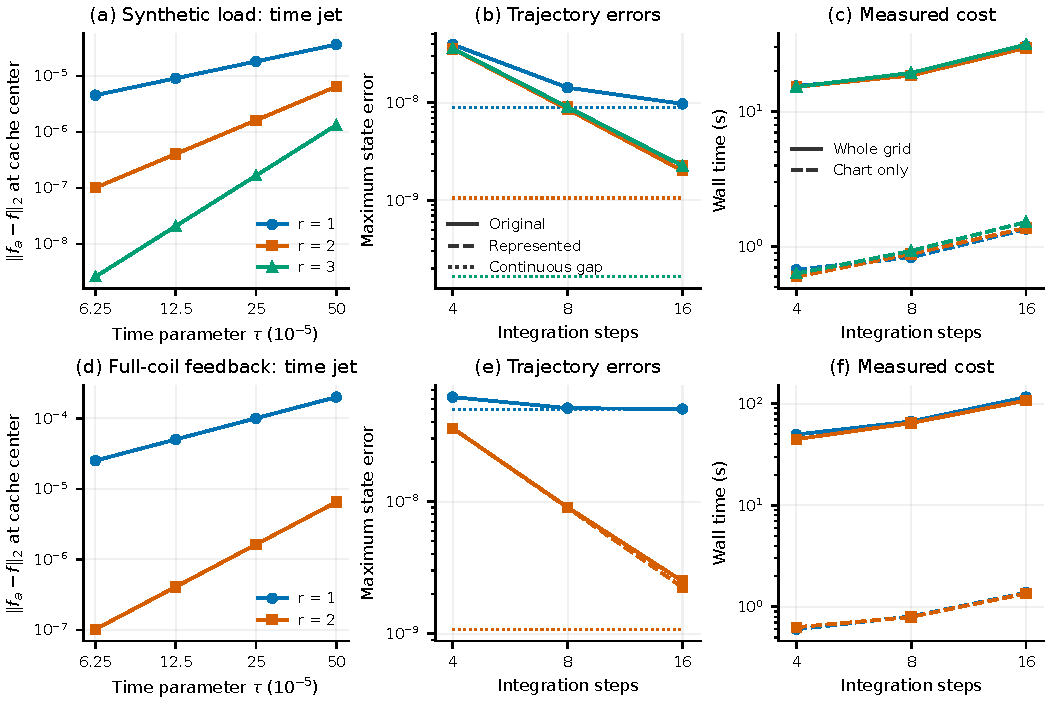
\includegraphics[width=\textwidth]{../figures/transport.pdf}
\caption{Accepted transport calculations. Rows correspond to the synthetic
load and full-coil collocated feedback. Left: native time-jet discrepancy at the
fixed cache center. Middle: sampled trajectory errors against the original
(solid) and represented (dashed) fields; dotted lines show continuous reference
gaps. Curves of represented errors nearly coincide. Right: complete grid wall
time and its auxiliary-chart component; coefficient and reference construction
are outside these per-grid timings. Color and marker identify transport order,
which does not change midpoint's second-order time discretization.}
\label{fig:transport}
\end{figure*}

\subsection{Direct integrators and failure domains}

Each direct-integrator branch has its own physical field and two independent
DOP853 references, using tolerances $(2\times10^{-11},2\times10^{-13},T/4)$
and $(5\times10^{-13},5\times10^{-15},T/8)$. Their reference refinement
differences are $1.24\times10^{-17}$, $8.01\times10^{-18}$, and
$1.38\times10^{-17}$ for fixed current, proportional drag, and collocated
feedback. All methods start at the same prescribed amplitude $0.01$, but errors
are compared only within a branch. The 15 method/grid combinations and 6
references took $690.713$\,s.

In the fixed-current conservative branch, midpoint and inherited nonseparable
Central4 attain finest errors $2.2449\times10^{-9}$ and
$1.4749\times10^{-13}$, with orders $1.9996$ and $3.9966$
(Figure~\ref{fig:integrators}). For synthetic proportional drag $-0.2P$, ordinary
and weighted midpoint are both second order, but only the weighted construction
targets $K(\tau)=e^{0.2\tau}K_0$. Its finest defect is
$1.11\times10^{-15}$, compared with $1.17\times10^{-9}$ for ordinary midpoint.
The actual collocated current law is evaluated at the unknown midpoint with
its full feedback Jacobian. Its canonical defect is $3.93\times10^{-4}$:
small integration residuals do not imply preservation of $K_0$. Central4 and
the proportional weighting are not applied to this general feedback branch.
Structure diagnostics use ideal implicit tangents at all midpoint steps, but
only the first Central4 step; floating-point maps are not asserted exactly
symplectic.

Locality is tested explicitly. Among 25 time-parameter chart probes, synthetic
order two at $\tau=0.2$, order three at $0.05$ and $0.2$, and full-coil order two
at $0.2$ leave the declared radius $0.002$ and are rejected. Two additional
outside-ball inputs are rejected as expected. These are auxiliary-chart probes,
not long robot trajectories. Polynomial nondegeneracy bounds lack directed
rounding and therefore are not interval certificates. The evidence establishes
short-window, smooth-field numerical connections; it does not establish chart
transitions, constrained sampled-feedback structure, long-time convergence, or
a new KAM certificate.

\begin{figure*}[t]
\centering
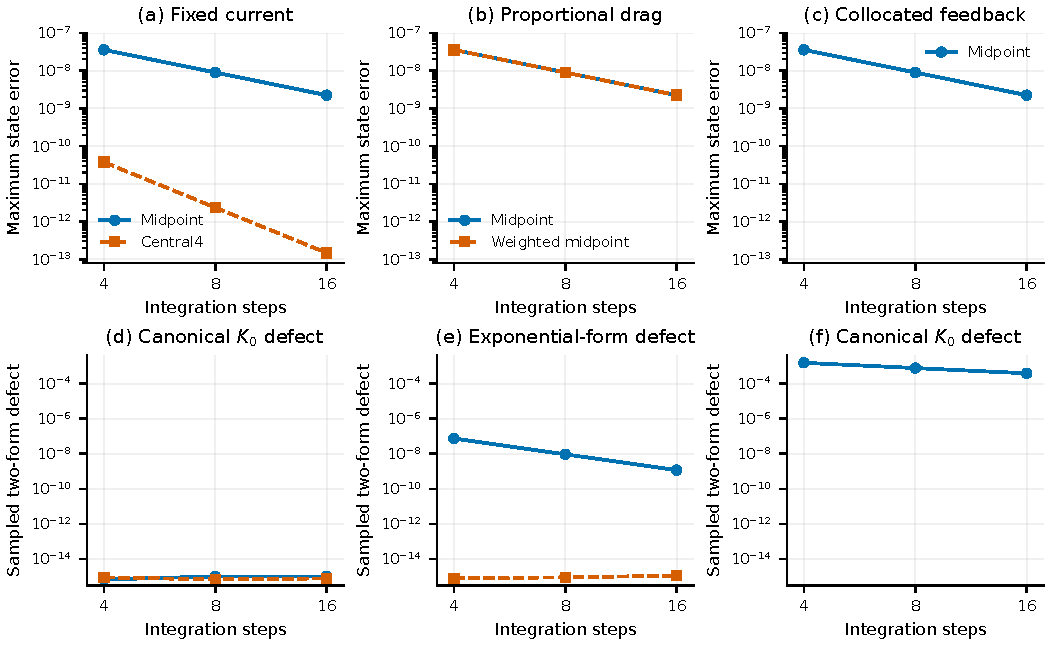
\includegraphics[width=\textwidth]{../figures/integrators.pdf}
\caption{Branch-specific direct integration. Top: errors against each branch's
own refined reference. Bottom: canonical two-form defects for fixed current and
collocated feedback, and the exponential two-form defect for proportional drag.
The two proportional-branch error curves nearly overlap. Defects sample ideal
implicit tangents, with only the first step sampled for Central4. The collocated
branch's nonzero canonical defect motivates a field-specific representation;
it does not invalidate its second-order trajectory convergence.}
\label{fig:integrators}
\end{figure*}

\section{Full-coil validation and transfer to the spatial rod}
\label{sec:physical-results}

\subsection{Energy-consistent forces can still invalidate an affine plant}
Independent checks establish consistency of the coil interface before evaluating control. For the final coil kernel and force allocator, geometric virtual work and differentiated magnetic energy differ by $4.44\times10^{-16}$ in the canonical force norm. Twelve-direction energy differences with perturbations $2\times10^{-6}$ and $10^{-6}$ give errors $3.70\times10^{-10}$ and $7.04\times10^{-10}$. An axial circular-loop closed form checks absolute SI units to relative error $3.90\times10^{-16}$; sampled divergence and curl defects are below $1.58\times10^{-17}$\,T\,m$^{-1}$. Changing loop quadrature from 128 to 256 to 512 points changes the force by at most $3.69\times10^{-16}$. These local floating-point checks support the implemented energy/force interface, without certifying a continuous operating domain.

The resulting full-coil force nevertheless differs substantially from the affine field having the same origin field, gradient, and total currents. Table~\ref{tab:coil-quadrature} and Figure~\ref{fig:coil} compare the same physical Ritz coefficients, pulling all forces back to the 20-cell canonical coordinates. The approximately 98.6\% relative discrepancy persists with spatial refinement. It is therefore not explained by loop integration error or solely by the single magnetic point of the coarse geometry. Absolute full-force differences remain $0.00586672$ and $0.00145763$ between consecutive spatial grids; the 20-cell approximation is not spatially converged. The rank increase also shows why quadrature-dependent reachability must be measured, rather than inferred from the number of current channels.

\begin{table}[t]
\centering
\caption{Common-configuration coil-force and reachability diagnostics. Relative force error is $\|F_{\rm full}-F_{\rm affine}\|/\|F_{\rm full}\|$; current-port rank uses relative threshold $10^{-8}$.}
\label{tab:coil-quadrature}
\begin{tabular}{@{}rrrr@{}}
\toprule
\shortstack{Spatial\\cells} & \shortstack{Magnetic\\points} & \shortstack{Relative\\force error} & \shortstack{Rank of\\$G_I$}\\
\midrule
20 & 1 & 0.985235663 & 5\\
40 & 2 & 0.985978752 & 7\\
80 & 4 & 0.986182968 & 7\\
\bottomrule
\end{tabular}
\end{table}

\begin{figure*}[t]
\centering
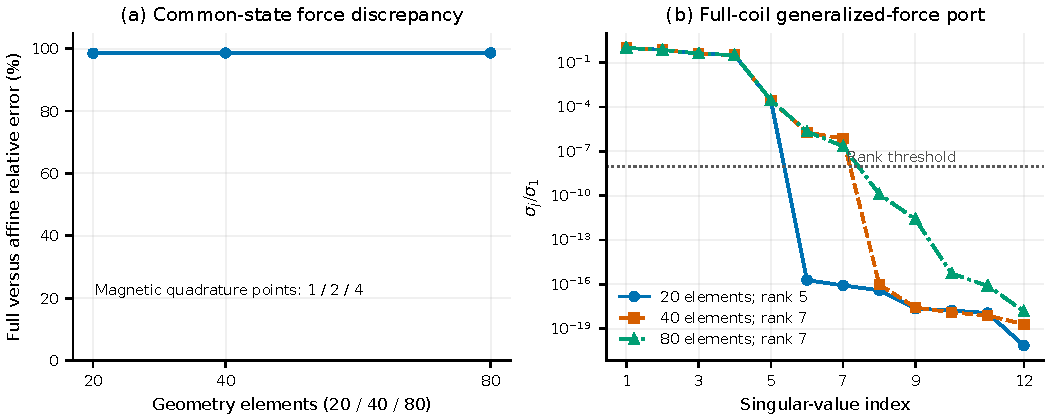
\includegraphics[width=\textwidth]{../figures/coil.pdf}
\caption{Full-coil force discrepancy and normalized current-port singular values at the same physical Ritz coefficients $q$ for 20/40/80 spatial quadrature cells. All forces and ports use the common 20-cell canonical basis. Magnetic quadrature has 1/2/4 active points. The persistent approximately 98.6\% affine discrepancy and numerical ranks 5/7/7 at relative threshold $10^{-8}$ preclude interpreting twelve coil channels as twelve independent generalized forces.}
\label{fig:coil}
\end{figure*}

For $d=0.2P_0$ and a $0.1$\,ms allocation interval, the orthogonal unreachable residual is $2.65530\times10^{-4}$ and the constrained residual is $4.01583\times10^{-4}$, with the 20\,A\,s$^{-1}$ limit active. Increasing this target by factors 10 and 100 gives constrained residuals $0.00500641$ and $0.07305644$. Correct feedback differentiation has directional finite-difference error $2.40\times10^{-9}$; differentiating the composed Hamiltonian instead changes the field by $5.47301$, while freezing feedback omits a Jacobian contribution of spectral norm $12.56491$. These are distinct implementation errors with direct consequences for an implicit closed-loop update.

\subsection{Actual constrained trajectories and their resolution limit}
The controlled trajectories are independently integrated from the same $z_0=\operatorname{initial\_state}(0.01)$, total bias, material, gain, and constraints. With $\gamma=0.2$, eight control updates cover $\tau\in[0,0.004]$, or $0.89733794$\,ms. One or two RK4 substeps per update give 8- and 16-step grids. Each branch evaluates its own feedback and actual plant force; an affine trajectory is not reused as a full-field trajectory.

The full-plant/full-controller and affine-plant/affine-controller trajectories differ by $3.90705\times10^{-4}$ in maximum canonical state norm. Their coarse/fine differences are approximately $7.22\times10^{-8}$, so the plant approximation has a resolved effect. On the full plant, however, replacing the full controller with its affine counterpart changes the trajectory by only $7.17555\times10^{-8}$. This window does not resolve a performance benefit from the full-field controller design. All four branches, including force compensation, have total and mechanical energy--work residual magnitudes near $6.25\times10^{-11}$ on the fine grid. The largest sampled magnetic-point field and gradient are $0.501325$\,mT and $0.00431404$\,T\,m$^{-1}$. Force compensation reaches 20\,A\,s$^{-1}$, but leaves a maximum force residual about $4.01416\times10^{-4}$.

The final allocator starts the force objective from an independently verified feasible previous current. Its rerun changes the earlier successful compensation trajectory by at most $1.17\times10^{-12}$ and currents by $6.51\times10^{-10}$\,A. This agreement does not establish identical derivatives of the optimization algorithm. Recomputed 36-dimensional sampled maps with exactly matched initial bias have numerical ranks 28 and 36 for collocated projection and force compensation, respectively. Their condition numbers are $5.43\times10^{18}$ and $2.09\times10^5$ in the stated canonical/current coordinates. Mechanical-block defects relative to $K_0$ are $3.22749\times10^{-3}$ and $1.03008\times10^{-4}$. The force-allocation Jacobian changes by $1.77112\times10^{-4}$ between versions, chiefly in the current-output block, despite a terminal mechanical-state difference of only $1.04\times10^{-14}$. Thus successful feasible allocation and nearly identical trajectories do not establish a smooth, invertible, or symplectic sampled map.

\subsection{Environmental transfer: feasible execution without tracking improvement}
\begin{figure*}[t]
\centering
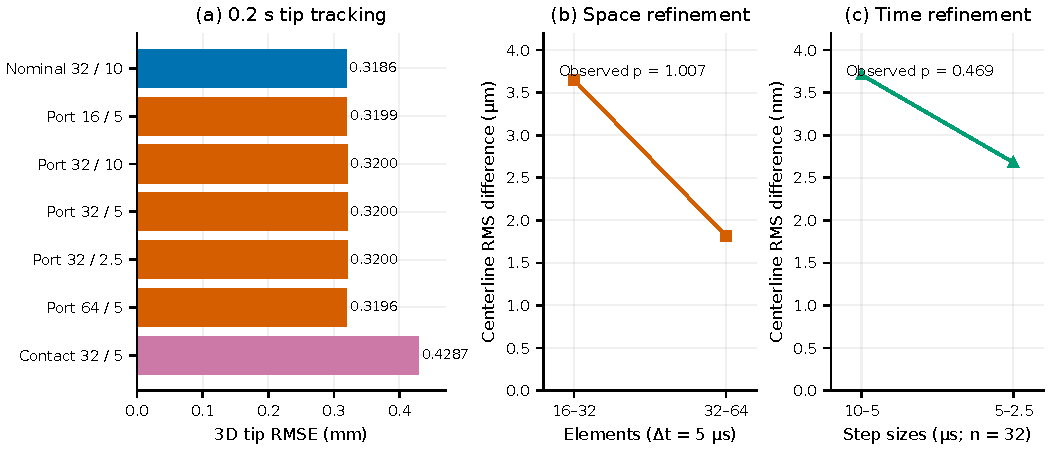
\includegraphics[width=\textwidth]{../figures/rod.pdf}
\caption{Spatial-rod transfer over 0.2\,s. Labels in (a) give the number of elements and time step in microseconds; nominal and port control are fairly compared at 32 elements and 10\,$\mu$s. The contact case is a separate 1.6\,mm-radius lumen geometry, whereas all other cases use the nominal 3\,mm lumen. Panels (b,c) show adjacent centerline differences at common times and 129 reference-arclength points. Observed rates describe these numerical differences and do not establish exact PDE error or second-order temporal convergence.}
\label{fig:rod}
\end{figure*}
Seven spatial-rod runs use the full coil forces and the physical gain in \eqref{eq:port-units}, over $0.2$\,s from a straight stationary state and zero actual current. This horizon ends before the $0.3$\,s target ramp completes. The implementation uses PyElastica PositionVerlet with the environmental forces described above. On the matched 32-element, 10\,$\mu$s grid, nominal control gives tip RMSE $0.318558$\,mm and the added port feedback gives $0.320032$\,mm: tracking slightly worsens. The 32-element, 5\,$\mu$s port case gives $0.320033$\,mm, maximum current $1.67831$\,A, maximum slew 20\,A\,s$^{-1}$, zero ramp discontinuity, and zero recorded violation at the 387 fixed constraint samples. Saved-node full-field maxima are $0.279966$\,mT and $0.0223521$\,T\,m$^{-1}$. These finite samples do not certify a continuous workspace.

The nominal 3\,mm lumen does not activate contact. A separate 1.6\,mm-radius lumen starts without penetration and develops maximum penetration $61.6032$\,$\mu$m and total normal force $11.3524$\,$\mu$N, with RMSE $0.428689$\,mm. Figure~\ref{fig:rod} reports this stress case separately. Ideal incremental port power is nonpositive, but projected and ramp-start increments reach positive values $3.19262\times10^{-8}$ and $3.20376\times10^{-8}$\,W. The 32-element, 5\,$\mu$s mechanical energy--work residual is $1.24636\times10^{-14}$\,J. Accurate accounting therefore coexists with loss of the ideal executed-input dissipation guarantee.

The original allocator fallback introduced an approximately $0.133$\,A discrepancy and spoiled temporal refinement. The final implementation clips to the current boxes and analytically repairs along a segment from the previous feasible current; it retains all nonconverged optimizer statuses. The seven final cases have zero fallbacks, 99 repairs each, and one to four nonconverged statuses, so feasibility is not presented as proven optimality. Adjacent centerline RMS differences at 129 common arclength points are $3.64802/1.81514$\,$\mu$m for 16/32/64 elements and $3.70928/2.67939$\,nm for 10/5/2.5\,$\mu$s steps. Observed spatial and temporal rates are $1.00703$ and $0.469234$, respectively; neither exact PDE error nor second-order temporal convergence is established.

Finally, a separate 2\,ms conservative comparison matches initial state, material, and fixed currents while disabling flow, wall, gravity, and damping. ROM-to-rod centerline RMS differences increase from $7.85933$ to $11.2030$ to $14.1690$\,nm across 16/32/64 elements; the corresponding tip RMS differences are $33.4755$, $65.6852$, and $86.4209$\,nm. Ritz truncation, shear/stretch restrictions, quadrature, and base-frame discretization remain distinct model errors. Its fixed currents also produce a full-rod gradient of $0.798394$\,T\,m$^{-1}$, exceeding the $0.03$\,T\,m$^{-1}$ limit. This diagnostic is not a feasible navigation result or a converged ROM error certificate.

\section{Learning Hamiltonians and resolving resonance}
\label{sec:learning-kam}

\subsection{A real energy with complex trainable representations}
Hamiltonian learning differentiates a scalar energy to obtain the conservative field \citep{Greydanus2019,Chen2022}. Here its target is the 12-configuration, 24-phase-dimensional variable-mass Kirchhoff model with 20 geometric integration cells and an ideal uniform axial magnetic bias, denoted by $H_{\mathrm{ideal}}$. The complete coil plant has a different magnetic potential. Fluid, contact and damping forces are excluded from these conservative labels. Thus learning tests approximation of the declared mechanical energy; its deployment additionally requires the physical port interface.

Use the dimensionless canonical state $z=(Q,P)$ and energy $h=H/E_0$, with $\tau=\omega_0t$. After the physical canonical scaling, define
\begin{equation}
 \begin{aligned}
 \xi&=(Q+iP)/\sqrt2,\\
 \chi&=(Q-iP)/\sqrt2.
 \end{aligned}
 \label{eq:learn-complex-coordinate}
\end{equation}
On the real slice $\chi=\bar\xi$; in a holomorphic extension they are independent. The inverse change of variables gives
\begin{equation}
 \begin{aligned}
 \partial_\chi&=(\partial_Q+i\partial_P)/\sqrt2,\\
 \{\xi_j,\chi_k\}&=-i\delta_{jk},\\
 \xi'&=-ih_\chi+iR/\sqrt2,
 \end{aligned}
 \label{eq:learn-complex-field}
\end{equation}
where $R$ enters the momentum equation. The same derivative convention must enter both the training loss and the predictor. Complex parameters do not make the physical energy complex-valued, and an imaginary energy output alone does not implement physical Rayleigh damping.

For training, $x=Dz$, where $D=\operatorname{diag}(\sqrt\nu,\sqrt\nu)/a$, $\nu=\omega/\omega_0$, and $a=0.08$. This additional scaling is not canonical: $\nabla_zh=D\nabla_xh$ and $x'=DJD\nabla_xh$. All models add a residual $r_\theta$ to the same quadratic prior $h_2=a^2\|x\|^2/2$.

The finite analytic model spans every cubic and quartic mechanical residual with momentum degree zero or two: $Q^3$, $Q^4$, $QP^2$, and $Q^2P^2$, contributing respectively 364, 1365, 936, and 6084 coefficients. These 8749 real parameters describe the stated mechanical class, rather than all quartics in 24 variables. The full complex network has two width-48 complex hidden layers and a complex readout, totaling 3552 complex or 7104 real parameters. It uses both complex inputs and conjugates, split activation $\sigma(u)=\tanh(\operatorname{Re}u)+i\tanh(\operatorname{Im}u)$, a cubic gate, and averaging over $P\mapsto-P$. All real and imaginary weights are trained. The gate preserves the quadratic prior; the averaging preserves momentum parity. Neither ensures convexity in momentum.

The mechanical complex network uses 13440 real parameters and predicts a lower-triangular matrix $L(Q)$ with positive exponential diagonal and $L(0)=I$, together with a potential residual. Its energy is
\begin{equation}
 \begin{aligned}
 h_\theta&=\tfrac12a^2x_P^TLL^Tx_P\\
 &\quad+\tfrac12a^2\|x_Q\|^2+V_\theta(x_Q),\\
 (h_\theta)_{PP}&=D_\nu LL^TD_\nu,
 \end{aligned}
 \label{eq:learn-spd}
\end{equation}
where $D_\nu=\operatorname{diag}\sqrt\nu$. For finite real outputs, $v^T(h_\theta)_{PP}v=\|L^TD_\nu v\|^2>0$ for every $v\ne0$. Hence the fixed-$Q$ momentum-to-velocity map is a linear bijection in exact arithmetic. This establishes structure without a uniform conditioning or physical mass-error bound.

Split activation is real analytic but not holomorphic in one complex argument. A valid extension replaces conjugate inputs by independent variables and uses
\begin{equation}
 \begin{aligned}
 \sigma^{\mathbb C}(u,v)&=\tanh((u+v)/2)\\
 &\quad+i\tanh((u-v)/(2i)),
 \end{aligned}
 \label{eq:learn-analytic-extension}
\end{equation}
with trained coefficients and their conjugates frozen. This gives a local holomorphic extension on domains avoiding all layer poles. No common pole margin or complex-domain approximation norm is certified by the reported training.

\subsection{Frozen training and mechanical diagnostics}
The experiment uses 1024 training and 256 validation states sampled uniformly in $[-1,1]^{24}$ with data seed 51001. Each architecture is trained with seeds 51001--51003, 1200 Adam updates and batch size 128. Learning rates are $10^{-3}$ for the polynomial and $3\times10^{-3}$ for the networks; the gradient clipping threshold is 10. With $r_*=h_{\mathrm{ideal}}-h_2$, the actual objective is
\begin{equation}
 \begin{aligned}
 \mathcal L&=\operatorname{mean}\left[\left(\frac{D(\nabla_xr_\theta-\nabla_xr_*)}{s_g}\right)^2\right]\\
 &\quad+0.15\operatorname{mean}\left[\left(\frac{r_\theta-r_*}{s_h}\right)^2\right],
 \end{aligned}
 \label{eq:learn-objective}
\end{equation}
where $s_h=0.00954395736$ is the training residual-energy standard deviation and $s_g=0.4661470702$ is its canonical-gradient RMS. Validation selects checkpoints every 50 updates, also checking the first update. All nine weights are frozen before generating 512 independent test labels in $[-1,1]^{24}$ and 256 wider-domain labels in $[-1.5,1.5]^{24}$ using seed 510990. Computation uses float64/complex128, one CPU thread and PyTorch 2.5.1; the recorded invocation takes approximately 410.8\,s.

Table~\ref{tab:learn-errors} and Figure~\ref{fig:learning} report the canonical-field relative $L^2$ error, $\|J\nabla(h_\theta-h_*)\|_2/\|J\nabla h_*\|_2$, over each sample set. The unrestricted complex network is most accurate under this budget, whereas the SPD model alone guarantees positive momentum curvature. The quadratic prior gives 63.094\% test error; a smaller historical 48-feature readout gives 62.964\%. Parameter counts, function classes, learning rates and per-update costs differ. These comparisons do not isolate an advantage of complex over real parameterization. In particular, finite-budget Adam does not establish the least-squares optimum of the polynomial class.

\begin{table*}[t]
 \centering
 \caption{Frozen learning results: ranges over three seeds. The last column counts nonpositive momentum Hessians at eight prescribed test states for each seed. Wider-domain samples use a 1.5-fold coordinate box.}
 \label{tab:learn-errors}
 \small\setlength{\tabcolsep}{3.5pt}
 \begin{tabular}{lrrrr}
 \toprule
 Model & Real parameters & Test field error (\%) & Wider-domain error (\%) & Nonpositive $h_{PP}$ \\
 \midrule
 Mechanical polynomial & 8749 & 35.249--35.282 & 59.743--60.273 & 4/4/4 \\
 Full complex hidden layers & 7104 & 3.241--3.700 & 8.410--9.063 & 2/2/4 \\
 SPD mechanical complex & 13440 & 11.415--11.553 & 20.651--21.917 & 0/0/0 \\
 \bottomrule
 \end{tabular}
\end{table*}

At eight test and eight wider-domain states per seed, we separately evaluate Hessians, energy second differences, and the Legendre equation $\partial_Ph_\theta(Q,\widehat P)=\partial_Ph_*(Q,P)$. Initialization at the true $P$ makes this a favorable local test. A small equation residual can coexist with a large recovered-momentum error. Some solver progress flags are false despite residuals near roundoff; the unrestricted complex model also has genuinely non-negligible inversion residuals. Its maximum sampled test Hessian condition number reaches $1.67\times10^5$. The SPD model's sampled wider-domain condition number reaches approximately 1811; positivity does not establish accurate inertia. The maximum sampled test Hessian relative errors are 47.49\%, 5.82\% and 17.05\%, and maximum relative recovered-momentum errors are 27.30, 0.6267 and 0.5044 for polynomial, complex and SPD models, respectively. Independently regenerated labels and directional second differences confirm the saved negative-curvature signs.

For deployment, the desired correction to the learned field is $(-\delta g_P,+\delta g_Q)$, with $\delta g=\nabla h_\theta-\nabla h_*$. Coil currents directly alter only the momentum equation. A separate constrained allocation therefore tests the reachable part of $\delta g_Q$ while retaining the configuration-velocity error and the force component outside the coil image. Across three models, three seeds and eight states, all 72 corrected allocations finish; effective port rank is five at relative cutoff $10^{-8}$, and some currents reach the 2\,A boundary. The after/before total-field-error ratios are 0.8845--0.9898, 0.8959--0.9960 and 0.8482--0.9965 for polynomial, complex and SPD models. This is a static allocation diagnostic with a declared 0.25\,s current-change window. It does not integrate a learned closed loop.


\begin{figure*}[t]
\centering
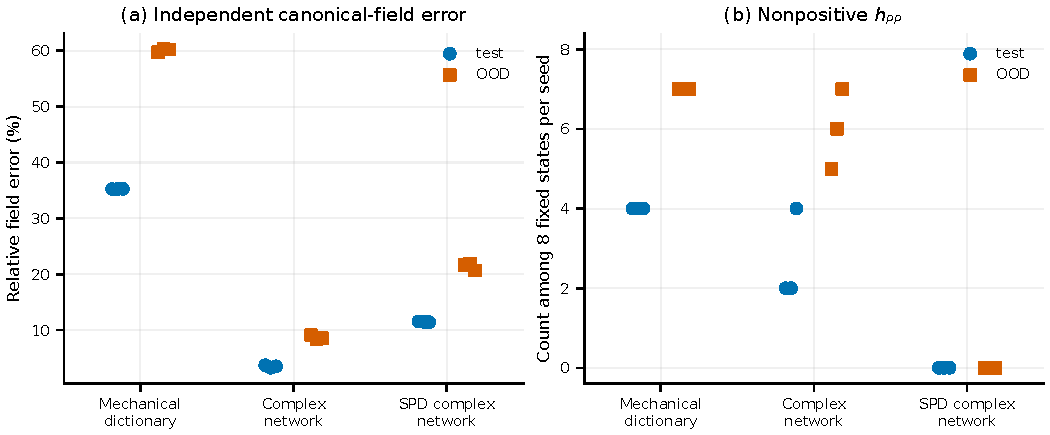
\includegraphics[width=\textwidth]{../figures/learning.pdf}
\caption{Frozen Hamiltonian-learning comparison. Each point denotes one of three training seeds; the left panel gives independent test and wider-domain canonical-field errors. The right panel counts nonpositive momentum Hessians among eight prescribed states per seed in each split. These finite samples are not uniform domain bounds. All models were trained on the ideal-bias Hamiltonian, not the full-coil potential.}
\label{fig:learning}
\end{figure*}

\subsection{From empirical error to a persistence hypothesis}
Two distinct error arguments preserve the learning-to-dynamics connection. For a finite basis, write $h_\theta=h_0+\sum c_{\theta j}\psi_j$ and $h_*=h_0+\sum c_{*j}\psi_j+R$. Stack sampled derivative features into $A$, remove the constant gauge, and use the same observation normalization $N_o$ for all residuals. If $G=A^TA/N_o\succeq\lambda I$, then
\begin{equation}
 \begin{aligned}
 \|h_\theta-h_*\|_{\mathcal X}
 &\le B_{\mathcal X}\frac{r+e}{\sqrt\lambda}+\|R\|_{\mathcal X},\\
 B_{\mathcal X}&=\Big(\sum_j\|\psi_j\|_{\mathcal X}^2\Big)^{1/2}.
 \end{aligned}
 \label{eq:learn-gram-bound}
\end{equation}
Here $r$ is the fitted observation residual and $e$ includes observation error and sampled derivatives of $R$. The proof uses the least singular value and Cauchy--Schwarz; it requires neither independent samples nor optimal fitting. The norm may be real $C^\ell$ or analytic supremum on a specified complex domain. Integral observations require their endpoint and quadrature errors, and exported coefficients require rounding bounds. The old two-mode full-cosine model retained all 35 quartic directions, realized by a cosine coefficient and 34 orthogonal polynomial directions. Its Gram bound does not transfer to the new 8749-feature dictionary.

A second, conditional argument \citep{Chen2022} combines parameter covering, Hoeffding concentration, Poincar\'e and interpolation. Let $\mathcal D=\mathbb T^n\times B$, $d=2n$, $p>d$, $\ell\ge1$, and integer $s>\ell+d/p$. Require independent samples with density at least $m_0$, a bounded realified parameter cube, uniformly bounded gradient residuals and parameter Lipschitz constant, and a uniform gauge-fixed $W^{s,p}$ bound $M_s$. Then, with probability at least $1-\delta$, simultaneously for the class,
\begin{equation}
 \begin{aligned}
 \|e_\theta\|_{C^\ell}&\le E_\theta,\\
 E_\theta&=C_{\mathrm{GN}}(G_\theta+M_s^\alpha G_\theta^{1-\alpha}),\\
 \alpha&=\frac{\ell-1+d/p}{s-1},
 \end{aligned}
 \label{eq:learn-statistical-bound}
\end{equation}
where $G_\theta=C_Pm_0^{-1/p}(\widehat R_\theta+\Gamma)^{1/p}$ and $\Gamma$ is the explicit covering penalty derived in the Supplement. This is a uniform statistical implication, not an Adam convergence theorem. Neither argument has all its constants certified for the present networks. Finite sampled gradient errors alone cannot supply them: already in one scalar variable $w$, the polynomial $c\prod_j(w-w_j)^2$ preserves zero values and first derivatives at the sample points while its complex-domain norm can grow arbitrarily with $c$.

\begin{figure*}[t]
\centering
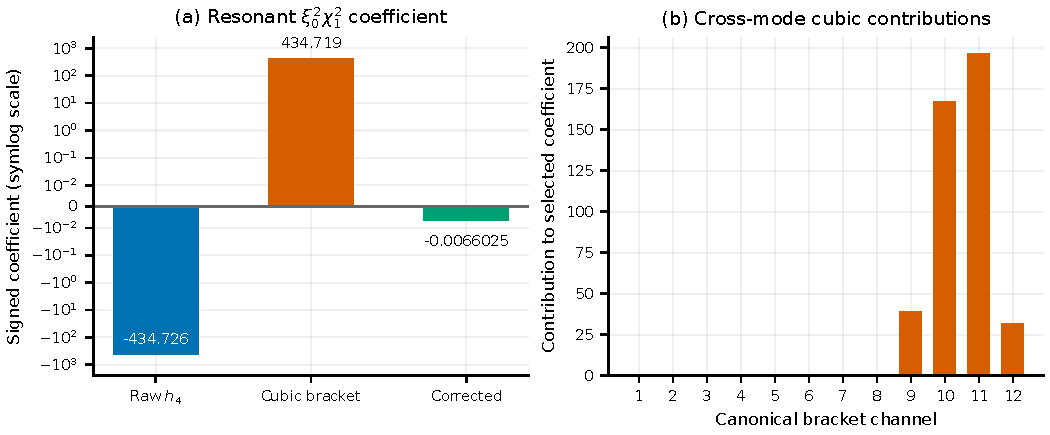
\includegraphics[width=\textwidth]{../figures/resonance.pdf}
\caption{First-pair quartic resonance diagnostic. Left: raw quartic coefficient, all-12-channel cubic-elimination correction and their small residual on a symmetric logarithmic scale. Right: the contributions of four external torsional bracket channels to the cubic-elimination correction, with channel indices numbered from one. All 12 canonical channels are retained in the computation. The original first-pair subspace is not invariant, so this restricted coefficient does not establish full-dimensional KAM nondegeneracy.}
\label{fig:resonance}
\end{figure*}

\subsection{The resonant three-dimensional mechanical model}
The actual linearized ideal-bias model has four $1{:}1$ bending pairs with frequency ratios $1$, $6.21276315$, $17.89814255$ and $80.07400435$. At cutoff $10^{-10}$, enumeration of all 2600 cubic monomials finds no resonances and minimum divisor one; among 17550 quartics, 206 lie in the homological kernel, including 78 action terms and 128 non-action terms. The paired degeneracy follows from circular-rod axial symmetry; the numerical cutoff is only its finite-order diagnostic.

For $h=h_2+h_3+h_4+\cdots$, $h_2=\sum_j\nu_j\xi_j\chi_j$, the homological equation and its cubic solution are
\begin{equation}
 \begin{aligned}
 \{h_2,\xi^\alpha\chi^\beta\}
 &=i\nu\cdot(\alpha-\beta)\xi^\alpha\chi^\beta,\\
 (W_3)_{\alpha\beta}&=\frac{i(h_3)_{\alpha\beta}}{\nu\cdot(\alpha-\beta)}.
 \end{aligned}
 \label{eq:learn-homological}
\end{equation}
Thus $\{h_2,W_3\}=-h_3$, and the Lie expansion gives the resonant quartic
\begin{equation}
 Z_4=\Pi_{\mathrm{res}}\left(h_4+\tfrac12\{h_3,W_3\}\right).
 \label{eq:learn-resonant-quartic}
\end{equation}
For the restriction to the first bending pair, all 12 canonical bracket channels are retained. Differentiating the full gradient twice in the four selected real coordinates supplies every cubic monomial that can survive this restriction after one derivative; terms containing two external variables cannot contribute. Four external torsional channels provide the nonzero correction to the coefficient of $\xi_0^2\chi_1^2$:
\begin{equation}
 \begin{aligned}
 &-434.7256304212535+434.719027922014\\
 &\qquad\simeq-0.006602499239534154.
 \end{aligned}
 \label{eq:learn-cancellation}
\end{equation}
The cancellation exceeds four orders of magnitude (Figure~\ref{fig:resonance}). The accepted calculation uses reverse automatic differentiation, with quartic permutation defect $2.27\times10^{-13}$ and independent scalar-derivative checks. Its raw coefficient differs from radius extrapolation by $7.26\times10^{-7}$. An earlier mixed-mode derivative tensor failed permutation symmetry (defect 1738.9) and is excluded; the failed artifact remains preserved. These checks validate finite-order numerical consistency, without bounding analytic tails or roundoff through the cancellation.

The computed restriction satisfies, to coefficient defect $1.23\times10^{-13}$,
\begin{equation}
 \begin{aligned}
 Z_{4,\mathrm{pair}}&=A(I_0+I_1)^2+BL^2,\\
 L&=Q_0P_1-Q_1P_0,
 \end{aligned}
 \label{eq:learn-pair-form}
\end{equation}
where $I_j=\xi_j\chi_j$, $A=0.0004112209869572539$, $B=0.006602499239534154$. The unitary transformation $\xi_\pm=(\xi_0\mp i\xi_1)/\sqrt2$ has symplectic realification and actions $I_\pm=(N\pm L)/2$, $N=I_0+I_1$. Consequently its formal twist has eigenvalues $4A\simeq0.00164488$, $4B\simeq0.0264100$ and determinant $16AB\simeq4.34414\times10^{-5}$. Independent checks at 32 states give maximum action-identity error $8.67\times10^{-19}$. However, three states in the original first-pair coordinate subspace have external field norms 0.01643, 0.06573 and 0.26300. That subspace is not invariant under the full nonlinear dynamics. The calculation therefore establishes a restricted quartic candidate, not a two-degree-of-freedom physical subsystem or full-dimensional twist. A single axial $SO(2)$ momentum also cannot supply four independent symmetry reductions; regular reduction requires a free action and regular momentum level, which fail at the straight equilibrium.




\subsection{Continuous and discrete KAM scope}
Continuous persistence requires a conservative Hamiltonian on a specified canonical domain, an integrable principal part with a bounded inverse frequency map, sufficient regularity, boundary margins, a Diophantine bound $|k\cdot\omega|\ge\gamma|k|^{-\tau}$ for every $k\ne0$, and the smallness threshold of the chosen theorem \citep{Poschel2001}. If $h_*=h_0+P_*$ and $h_\theta=h_0+P_\theta$ in the same chart, a certified bound $\beta_\theta$ for the gauge-fixed learned perturbation and an error bound $E_\theta$ must together satisfy $\beta_\theta+E_\theta<c_K\gamma^2$ under the corresponding theorem's hypotheses. Applying the theorem separately gives two torus families, not identical embeddings. Physical perturbations and normal-form remainders remain in this budget.

Discrete persistence additionally requires an analytic exact-symplectic map and inverse on retained domains, a periodic generating function, discrete twist and frequency margins, and
\begin{equation}
 |e^{i\Delta k\cdot\omega}-1|\ge\Delta\gamma_D|k|^{-\tau_D}\quad(k\ne0).
 \label{eq:learn-discrete-divisor}
\end{equation}
The generating-function perturbation is normalized by $\Delta$ before comparison with a Hamiltonian bound \citep{Shang1999}. Small step size alone does not prevent $\Delta k\cdot\omega=2\pi m$. Exact implicit symplecticity also does not identify the finite-tolerance solver with an exact-symplectic map. The inherited finite-amplitude certificate concerns a particular frozen two-mode Hamiltonian, with its own Fourier candidate and verified-domain calculations; it supplies no certificate for either present three-dimensional magnetic potential. Full resonant coupling, inverse twist, domain and remainder bounds, and continuous/discrete small-divisor constants remain uncertified here.

\section{Discussion}
\subsection{What is connected, and what remains separate}
The reduction connects three-dimensional geometry, variable inertia, magnetic energy, a physical current port and implicit integration. On a smooth full-coil feedback branch, the same original field also supplies the transported-form and direct-midpoint comparisons. This is a concrete connection between mechanics and local structure. Its accuracy statement remains decomposed: a precisely matched chart for a truncated form need not integrate the original field precisely. The reported full-coil window is short, and the chart construction is substantially more expensive than the simulated physical duration.

The constrained sampled controller and environmental rod are further, distinct calculations. Their feasibility and power records do not inherit the exact-symplectic statement proved for the ideal conservative implicit map. Current memory, active constraints, interpolation and environmental loads change the mathematical object. Similarly, the learned networks approximate the ideal-bias energy, not the full-coil Hamiltonian. Static force allocation is the implemented learning-to-actuation diagnostic; no experiment here integrates the full learned controller through the local Birkhoff chart and then transfers that combined controller to the rod. This missing combined validation cannot be supplied by adding the successes of separate branches.

\subsection{Limitations of the physical and mathematical evidence}
The force discrepancy with an affine field is specific to the tested geometry and state. It establishes the need to check the approximation in use, rather than a universal lower bound on affine magnetic models. The full-coil result is itself subject to magnetic material assumptions and spatial quadrature error. The 12 current channels do not remove the measured force-rank deficiency. The short ROM control comparison resolves a plant-model difference, but not a tracking benefit from the controller change. The longer rod test slightly worsens tracking and has low observed temporal refinement order. Neither result supports a claim of improved navigation performance.

The physical application remains broader than the validated layers. The ROM transport calculations use smooth declared loads; they do not include pulsatile-flow/contact switching. The rod has prescribed flow and a rigid wall, with synthetic residual acceleration. Two-way fluid--structure coupling, deformable vessels, physiological boundary data, hardware-calibrated coils and microgravity validation are absent. The short conservative ROM-to-rod comparison does not bound model reduction error in a loaded vessel and even violates a full-rod gradient limit. Keeping this diagnostic prevents small state differences from being misinterpreted as feasible intervention.

The mathematical results are also local or conditional where stated. Uniform bounds for charts, inverse maps, derivatives and perturbations are not supplied by sampled defects. Frozen complex models lack a verified analytic-domain error budget, and their energy curvature failures restrict a mechanical interpretation. The resonant quartic calculation yields a candidate first-pair structure, but not a full invariant subsystem or a 12-action twist certificate. No continuous or discrete KAM theorem is applied to blood flow, contact, sampled constrained feedback, or the learned three-dimensional model.

\section{Conclusion}
A geometric three-dimensional rod can be connected to a computable local Birkhoff representation without freezing its mass, and to a realizable magnetic input without treating arbitrary phase corrections as actuation. The existing results quantify each connection and its limitations. Higher-order transport reduces representation error, conservative Central4 achieves the expected order, and full-coil virtual work agrees with magnetic-energy differentiation. These positive results coexist with substantial affine-force error, rank-limited control, nonconvex learned momentum energies, unresolved resonant persistence and no demonstrated rod tracking improvement. The resulting evidence supports local structure-aware simulation and a physically consistent actuator interface. It does not yet establish a unified learned, structure-preserving vascular controller or a three-dimensional KAM certificate.

\section*{Statements and declarations}
\paragraph{Authors and contributions.} Author names, affiliations, corresponding-author details and contribution statements must be supplied and approved by the responsible human authors before submission.
\paragraph{Funding.} Funding sources and grant identifiers have not been provided and must be completed by the authors.
\paragraph{Competing interests.} A declaration has not been supplied; the authors must complete it before submission.
\paragraph{Ethics and consent.} The reported study uses mathematical models and numerical simulations. No human-participant, patient or animal data are analyzed. Institutional requirements and the final declaration remain the authors' responsibility.
\paragraph{Data and code availability.} The source record is available at \url{https://github.com/mop74720-commits/1028}, Stage~5 commit \texttt{1c73a58} (full identifier in the accompanying README). The manuscript bundle includes source-field and SHA-256 manifests, figure-building code, frozen-data paths and bilingual supplementary proofs. Rebuilding the figures does not rerun the scientific experiments. Missing historical assets and rejected outputs are identified rather than reconstructed.
\paragraph{AI-assisted preparation.} OpenAI Codex assisted source inspection, manuscript organization, drafting, translation, data extraction, figure preparation and LaTeX compilation. It is not an author. The responsible authors must verify the mathematics, evidence, references and declarations and approve both language versions before submission. No new scientific experiment was generated for this manuscript preparation.

\bibliographystyle{sageh}
\bibliography{../references}
\end{document}
